 %!TEX root = ./template-skripsi.tex
%-------------------------------------------------------------------------------
%                            BAB II
%               KAJIAN TEORI
%-------------------------------------------------------------------------------

\chapter{KAJIAN PUSTAKA} 

\section{Pengertian \emph{Bates-Jensen Wound Assessment Tool}}

\emph{Bates-Jensen Assessment Tool} atau BWAT adalah alat ukur yang digunakan untuk menilai dan memantau penyembuhan luka tekan dan luka kronis lainnya. Pada tahun 1990, \textit{Bates-Jensen} mengembangkan PSST, yang direvisi pada tahun 2001 sebagai BWAT. PSST asli dikembangkan sebagai alat penilaian luka untuk penggunaan klinis dan penelitian. Selama bertahun-tahun, penggunaan BWAT telah berkembang untuk mengukur dan memprediksi penyembuhan luka dan digunakan dalam berbagai macam luka di luar ulkus dekubitus. BWAT telah memberikan dasar untuk banyak alat penilaian luka lainnya dan merupakan instrumen yang paling banyak digunakan. Hanya perubahan kecil yang dilakukan pada PSST untuk membuat alat generasi kedua, BWAT.

\section{Kegunaan \emph{Bates-Jensen Wound Assessment Tool}}

BWAT direkomendasikan untuk digunakan dalam menilai dan memantau penyembuhan luka tekan dan luka kronis lainnya. Ini menggunakan skala numerik untuk menilai karakteristik luka dari yang terbaik hingga yang terburuk (lihat Lampiran 5D). Dua item tidak dinilai: lokasi dan bentuk. 13 sisanya adalah item yang diberi skor. Ini adalah: ukuran, kedalaman, tepi, \textit{undermining} atau kantong, jenis jaringan nekrotik, jumlah jaringan nekrotik, jenis eksudat, jumlah eksudat, warna kulit di sekitarnya, edema jaringan perifer, indurasi jaringan perifer, jaringan granulasi, dan epitelisasi. Setiap item yang diberi skor muncul dengan deskriptor karakteristik yang dinilai pada skala (1 menunjukkan yang terbaik untuk karakteristik itu dan 5 menunjukkan yang terburuk). Setelah selesai dinilai untuk setiap item pada BWAT, 13 skor item dapat dijumlahkan untuk mendapatkan skor total untuk luka. Skor total kemudian dapat diplot pada rangkaian luka di bagian bawah alat untuk “melihat sekilas” penyembuhan atau degenerasi luka. Skor total berkisar dari 9 (penutupan luka) hingga 65 (degenerasi jaringan yang dalam). Alat ini memiliki lembar petunjuk penggunaan satu halaman, selain deskripsi item (Lampiran B). Ada juga panduan bergambar untuk melatih profesional kesehatan dalam menggunakan BWAT. Panduan Bergambar BWAT mencakup 102 foto dari berbagai jenis luka, bukan hanya luka tekan, yang menggambarkan setiap deskriptor untuk setiap item BWAT. Validasi konten fotografi dicapai dalam proses konsensus tiga tahap yang bekerja dengan perawat yang mengkhususkan diri dalam perawatan luka. Gambar 2.1 memberikan contoh halaman dari panduan bergambar.
\begin{figure}[H]
	\centering
	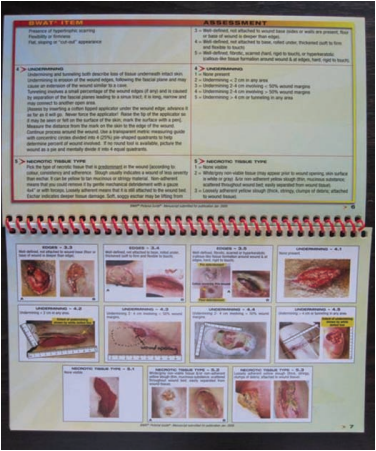
\includegraphics[keepaspectratio, width=8cm]{gambar/panduan_bergambar}
	\caption{Halaman dari panduan bergambar penilaian luka \textit{Bates-Jensen} \citep{sussman2012}}
	\label{gambar:bates_jensen_assessment_tool}
\end{figure}
Luka harus dinilai dengan BWAT pada awalnya untuk penilaian dasar dan secara berkala (yaitu, setidaknya setiap minggu) untuk mengevaluasi efektivitas intervensi.

\section{Penggunaan Skor BWAT untuk Mengidentifikasi Status Keparahan dan Panduan Perawatan}

Tingkat keparahan luka, serta status kesehatan pasien secara keseluruhan, dapat menentukan pendekatan manajemen yang tepat untuk penyembuhan. Status keparahan adalah ukuran derajat kerusakan jaringan atau beban luka pada pasien. Tujuan perawatan luka adalah untuk mengurangi status keparahan secara keseluruhan dan membuat penurunan ini tepat waktu. Perawat dapat menggunakan BWAT untuk membantu perawat mengidentifikasi tingkat keparahan luka, dan dengan demikian memandu perencanaan perawatan pasien.
Seperti yang ditunjukkan pada Gambar 2.2, skor BWAT dapat dibagi menjadi empat status keparahan yang disarankan: skor total 13-20 menunjukkan keparahan minimal; 21–30 menunjukkan keparahan ringan; 31-40 adalah tingkat keparahan sedang; dan 41-65 adalah tingkat keparahan yang ekstrim. Contoh algoritme perawatan untuk satu luka di masing-masing kondisi keparahan ini disajikan di bawah ini. Algoritma pengobatan ini berasal dari pedoman praktek klinis.
\begin{figure}[H]
	\centering
	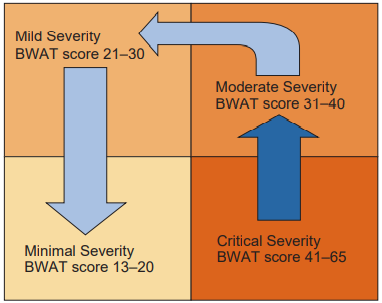
\includegraphics[keepaspectratio, width=8cm]{gambar/skor_tingkat_keparahan}
	\caption{Status keparahan berdasarkan skor BWAT. Tujuan terapi adalah (1) untuk mengurangi tingkat keparahan luka secara keseluruhan dan, dengan demikian, skor BWAT dan (2) untuk membuat penurunan secara tepat waktu. Ada perhatian yang sama mengenai tingkat keparahan luka dan durasi waktu yang dihabiskan luka dalam kondisi parah apa pun. \citep{sussman2012}}
	\label{gambar:skor_tingkat_keparahan_bwat}
\end{figure}
\begin{enumerate}
	\item Skor Tingkat Keparahan Minimal BWAT 13–20
	
	Luka dengan skor total BWAT 13-20 umumnya merupakan luka dengan ketebalan parsial yang dangkal. Gambar 5.23 menyajikan algoritme generik untuk perawatan luka dalam keadaan parah ini. Tujuan utama luka dalam keadaan parah ini adalah untuk mencegah kerusakan lebih lanjut dan menyediakan lingkungan luka yang lembab untuk penyembuhan.
	\item Skor Tingkat Keparahan Ringan BWAT 21–30
	
	Luka dengan tingkat keparahan ringan meliputi luka sebagian dan seluruh ketebalan. Gambar 5.24 menyajikan algoritme perawatan umum untuk luka dengan ketebalan parsial dengan skor keparahan ringan. Tujuan perawatan luka parsial dengan tingkat keparahan ringan adalah untuk menyerap eksudat luka yang berlebihan, mempertahankan dasar luka yang bersih, dan menjaga lingkungan yang lembab. Luka full-thickness dengan skor keparahan ringan menawarkan lebih banyak pilihan untuk pengobatan karena luka dapat muncul sebagai luka bersih, full-thickness atau sebagai luka yang diisi dengan puing-puing nekrotik.
	\item Skor Tingkat Keparahan Sedang BWAT 31–40
	
	Gambar 5.25 adalah rencana perawatan untuk luka full-thickness dengan jaringan nekrotik. Tujuan perawatan luka full-thickness dengan tingkat keparahan sedang adalah untuk mendapatkan/mempertahankan dasar luka yang bersih, menyediakan lingkungan yang lembab, menyerap eksudat berlebih, mencegah penutupan dini, dan mengurangi ruang mati luka. Luka dengan skor keparahan sedang (dan ringan) memiliki presentasi klinis yang paling beragam, sehingga pilihan mengenai pengobatan sangat banyak.
Gambar 5.26 sampai 5.28 menunjukkan algoritma pengobatan umum. Algoritma ini dapat digunakan untuk menentukan perawatan yang tepat untuk berbagai luka kronis dengan skor keparahan BWAT sedang hingga ekstrim. Luka dengan tingkat keparahan sedang sebagian besar merupakan luka full-thickness seperti ulkus dekubitus stadium III atau IV. Gambar 5.26 menyajikan kasus luka full-thickness dengan puing-puing nekrotik dan eksudat dalam jumlah besar. Perawatan difokuskan pada debridement dan penyerapan eksudat. Gambar 5.27 menyajikan kasus luka bersih full-thickness dengan undermining atau dead space, dan fokus pengobatan adalah menghilangkan dead space dan pencegahan penutupan luka prematur. Tujuan perawatan luka pada keadaan keparahan ini adalah untuk mendapatkan/mempertahankan dasar luka yang bersih, menyerap eksudat berlebih, menghilangkan ruang mati untuk mencegah penutupan luka prematur, dan menyediakan lingkungan luka yang lembab.
	\item Skor Tingkat Keparahan Kritis BWAT 41–65
	
	Luka dengan skor total BWAT antara 41 dan 65 umumnya merupakan luka full-thickness yang dalam dengan manifestasi klinis yang lebih kritis, termasuk undermining dan nekrosis. Gambar 5.28 menyajikan algoritma untuk perawatan luka dengan eskar nekrotik. Tujuan perawatan luka pada keadaan keparahan ini adalah untuk mengidentifikasi dan mengobati infeksi, mendapatkan dasar luka yang bersih, menyerap eksudat berlebih, menghilangkan ruang mati untuk mencegah penutupan luka prematur, dan menyediakan lingkungan luka yang lembab.
Pertimbangan dalam Menggunakan Skor BWAT untuk Memandu Perawatan
Penggunaan skor BWAT untuk menentukan keadaan keparahan dan membimbing pengobatan menawarkan satu pendekatan untuk mengelola luka. Pendekatan ini mungkin berguna dalam merancang pedoman pengobatan generik yang luas; namun, pasien tetap harus menggunakan penilaian klinis perawat untuk mengindividualisasikan rencana perawatan. Selain itu, rencana perawatan yang disajikan berdasarkan skor keparahan BWAT hanya berfokus pada perawatan luka topikal. Perhatian pada nutrisi, penggunaan permukaan penopang yang memadai, penentuan kebutuhan perawatan luka yang lebih lanjut, dan pertimbangan status seluruh pasien juga merupakan bagian dari rencana perawatan.
\end{enumerate}
\begin{figure}[H]
	\centering
	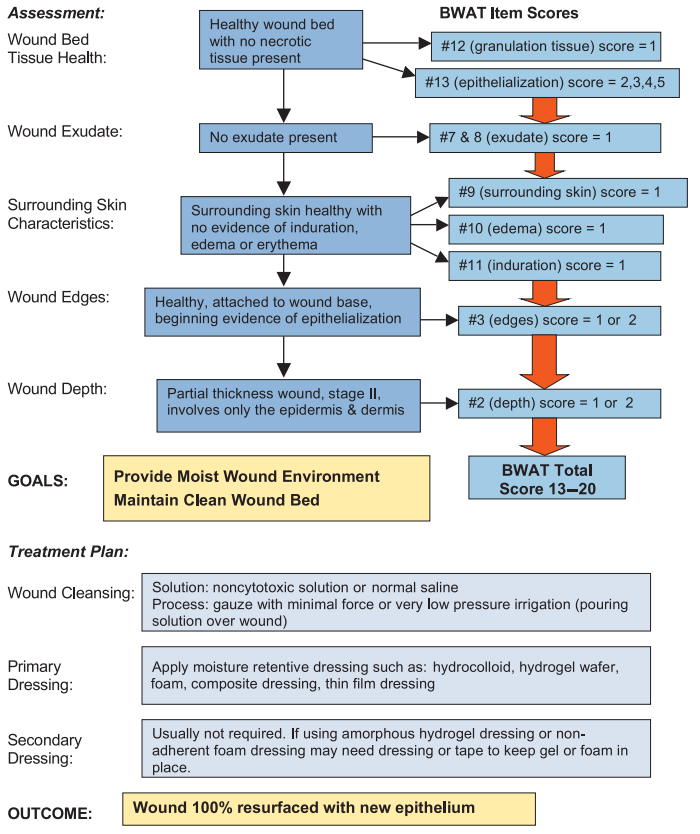
\includegraphics[keepaspectratio, width=14cm]{gambar/gambar_23}
	\caption{Algoritma perawatan skor keparahan BWAT minimal untuk luka ringan, kering, dengan ketebalan sebagian. (Diadaptasi dari ConvaTec, dengan izin.) \citep{sussman2012}}
	\label{gambar:gambar_23}
\end{figure}

\begin{figure}[H]
	\centering
	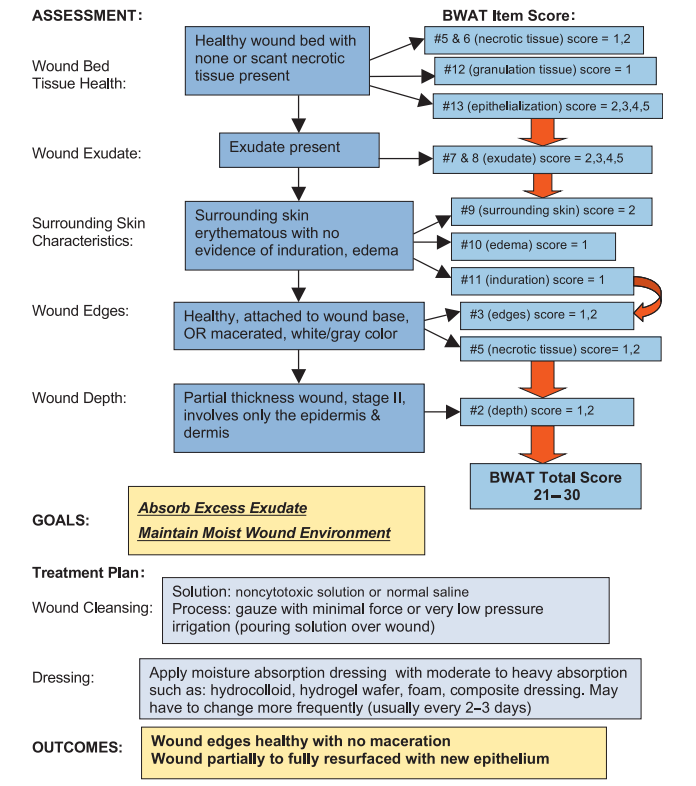
\includegraphics[keepaspectratio, width=14cm]{gambar/gambar_24}
	\caption{Parsial-ketebalan luka dengan algoritma pengobatan skor keparahan BWAT ringan. (Diadaptasi dari ConvaTec, dengan izin.) \citep{sussman2012}}
	\label{gambar:gambar_24}
\end{figure}

\begin{figure}[H]
	\centering
	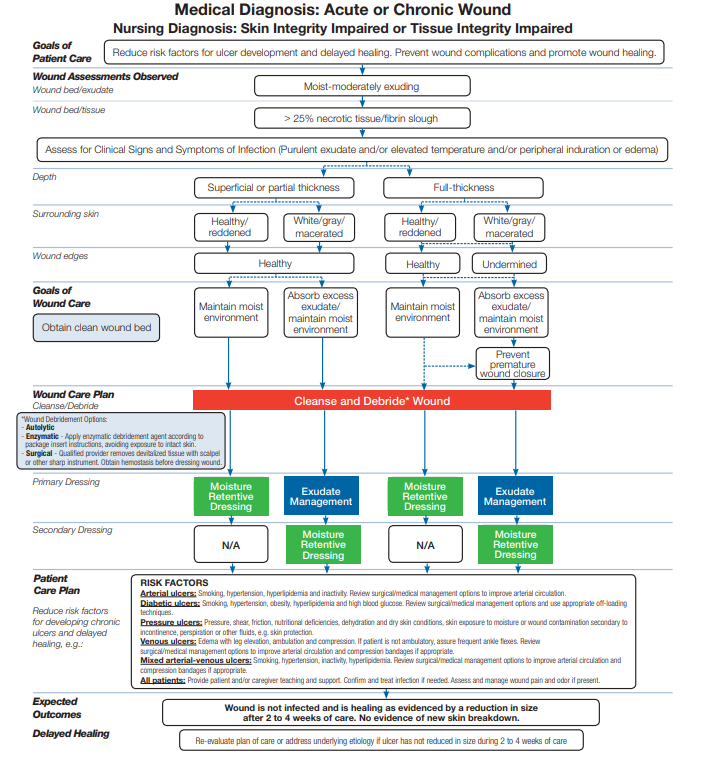
\includegraphics[keepaspectratio, width=14cm]{gambar/gambar_25}
	\caption{Ulkus tekan stadium III atau stadium IV dengan ketebalan penuh dengan algoritme pengobatan skor keparahan BWAT sedang. (Diadaptasi dari ConvaTec, dengan izin.) \citep{sussman2012}}
	\label{gambar:gambar_25}
\end{figure}

\begin{figure}[H]
	\centering
	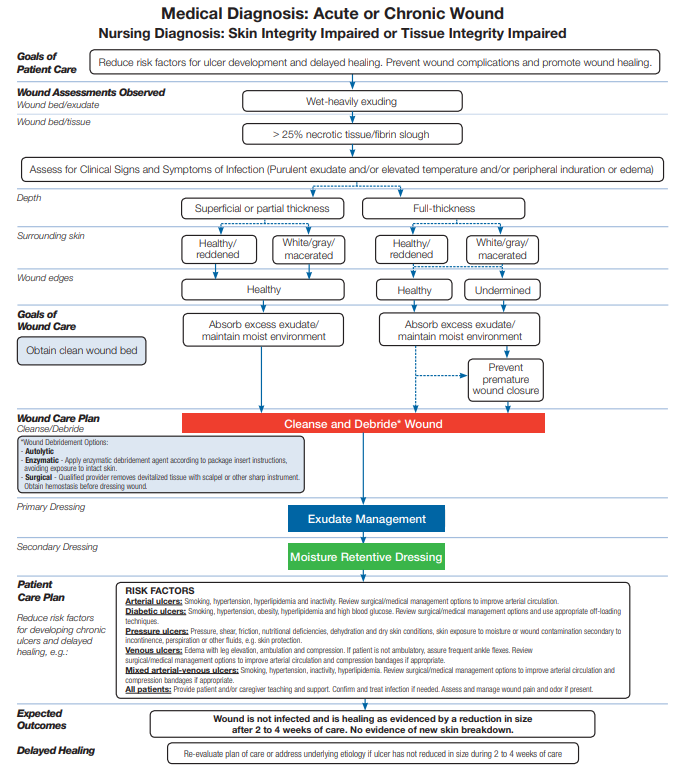
\includegraphics[keepaspectratio, width=14cm]{gambar/gambar_26}
	\caption{Luka dengan ketebalan penuh umum dengan algoritme perawatan skor keparahan BWAT kritis. (Dicetak ulang dari ConvaTec, dengan izin.) \citep{sussman2012}}
	\label{gambar:gambar_26}
\end{figure}

\begin{figure}[H]
	\centering
	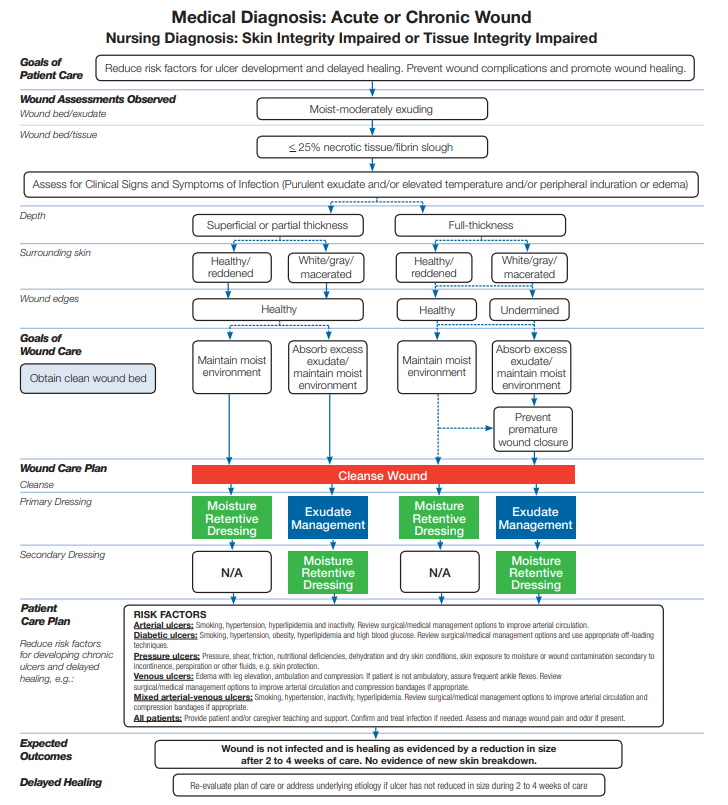
\includegraphics[keepaspectratio, width=14cm]{gambar/gambar_27}
	\caption{Luka dengan ketebalan penuh umum dengan \textit{undermining} atau \textit{pocketing} dengan algoritme perawatan skor keparahan BWAT sedang. (Dicetak ulang dari ConvaTec, dengan izin.) \citep{sussman2012}}
	\label{gambar:gambar_27}
\end{figure}

\begin{figure}[H]
	\centering
	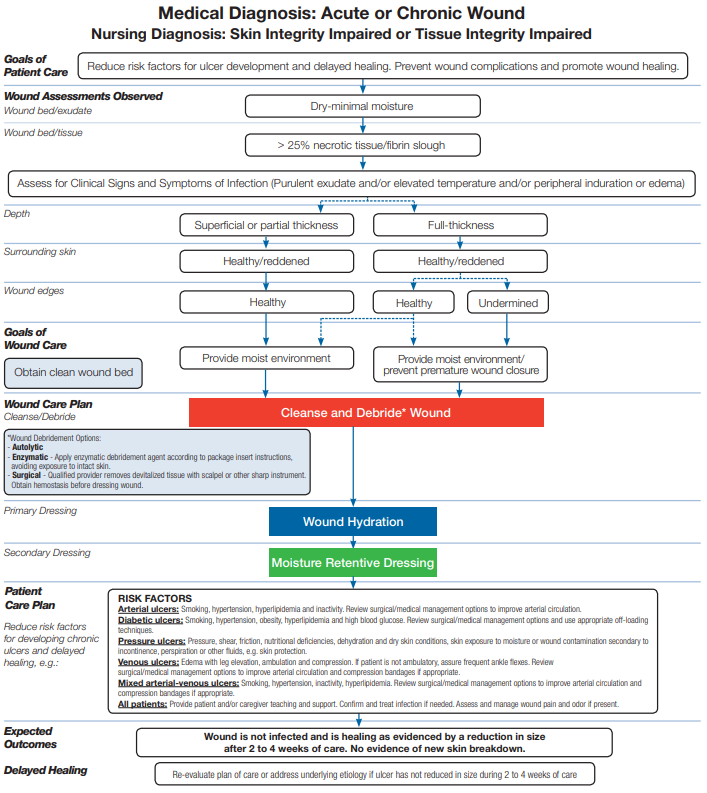
\includegraphics[keepaspectratio, width=14cm]{gambar/gambar_28}
	\caption{Skor keparahan BWAT kritis dengan algoritme perawatan eschar kering. (Dicetak ulang dari ConvaTec, dengan izin.) \citep{sussman2012}}
	\label{gambar:gambar_28}
\end{figure}

\section{\emph{Activity vs Fragment}}

\emph{Activity} adalah satu hal yang terfokus dapat dilakukan pengguna. Hampir semua \textit{activity} berinteraksi dengan pengguna, jadi \textit{class Activity} menangani pembuatan desain untuk menempatkan \textit{User Interface}(UI) dengan \textit{setContentView(View)}.
\textit{Fragment} mewakili bagian UI aplikasi yang dapat digunakan kembali. \textit{Fragment} mendefinisikan dan mengelola tata letaknya sendiri, memiliki siklus hidupnya sendiri, dan dapat menangani kejadian \textit{input}nya sendiri. \textit{Fragment} tidak dapat hidup sendiri, harus di\textit{hosting} oleh \textit{activity} atau \textit{fragment} lain.
Perbedaan utama yang muncul dari definisi di atas adalah bahwa \textit{fragment} bergantung pada \textit{activity} yang ada sehingga hanya mewakili sebagian UI. Sebaliknya, \textit{activity} dapat dianggap seperti wadah dimana semua komponen UI lainnya (termasuk \textit{fragment}) akan ditempatkan. Tanpa \textit{activity}, tidak akan ada \textit{interface} pengguna. Cara untuk membuat \textit{fragment} ialah:
\begin{enumerate}
\item \textit{Setup environment}

Fragment memerlukan dependency pada library AndroidX Fragment. Diperlukan menambahkan repositori Google Maven ke file settings.gradle proyek untuk menyertakan dependency
\begin{figure}[H]
	\centering
	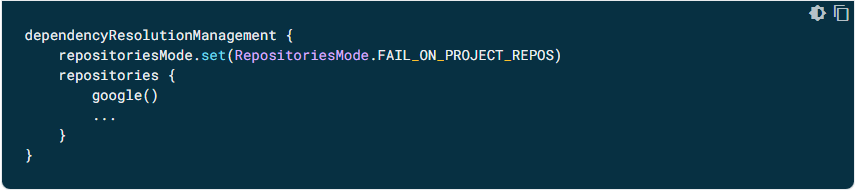
\includegraphics[keepaspectratio, width=12cm]{gambar/fragment_setup_environment1}
	\caption{Contoh menambahkan repositori \textit{Google Maven} pada \textit{dependency} \citep{developerandroid}}
	\label{gambar:gambar_29}
\end{figure}
Untuk menyertakan \textit{AndroidX Fragment} ke proyek, tambahkan \textit{dependency} berikut dalam file \textit{build.gradle}:
\begin{figure}[H]
	\centering
	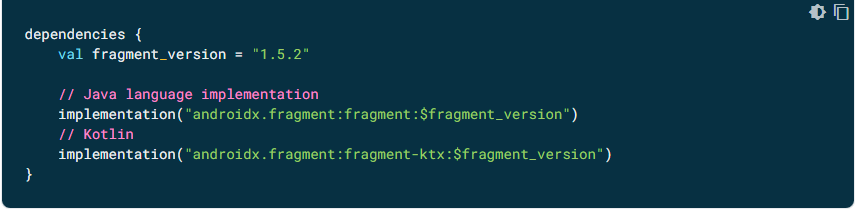
\includegraphics[keepaspectratio, width=12cm]{gambar/fragment_setup_environment2}
	\caption{Contoh menambahkan \textit{AndroidX Fragment} \citep{developerandroid}}
	\label{gambar:gambar_30}
\end{figure}
\item Buat kelas \emph{fragment}

Untuk membuat \textit{fragment}, perluas kelas \textit{AndroidX Fragment}, dan ganti metodenya untuk menyisipkan logika aplikasi, mirip dengan cara membuat kelas \textit{Activity}. Untuk membuat \textit{fragment} minimal yang menentukan \textit{layout}nya sendiri, berikan \textit{resource layout fragment} ke konstruktor dasar, contohnya sebagai berikut:
\begin{figure}[H]
	\centering
	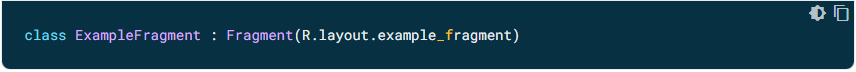
\includegraphics[keepaspectratio, width=12cm]{gambar/fragment_class}
	\caption{Contoh berikan \textit{resource layout fragment} ke konstruktor dasar \citep{developerandroid}}
	\label{gambar:gambar_31}
\end{figure}
\textit{Library fragment} juga menyediakan kelas dasar \textit{fragment} yang lebih khusus:
	\begin{enumerate}
	\item \emph{DialogFragment}
	
	Menampilkan dialog mengambang. Menggunakan kelas ini untuk membuat dialog adalah alternatif yang baik untuk menggunakan metode pembantu dialog di kelas Activity, karena fragment secara otomatis menangani pembuatan dan pembersihan dialog.
	\item \emph{PreferenceFragmentCompat}
	
	Menampilkan hierarki objek \textit{Preference} sebagai daftar. Kita dapat menggunakan \textit{PreferenceFragmentCompat} untuk membuat layar pengaturan untuk aplikasi.
	\end{enumerate}
\item Tambahkan \textit{fragment} ke \textit{activity}

Umumnya, \textit{fragment} harus disematkan dalam \textit{AndroidX FragmentActivity} untuk menyumbangkan UI ke \textit{layout activity} tersebut. \textit{FragmentActivity} adalah kelas dasar untuk \textit{AppCompatActivity}, jadi jika sudah membuat subkelas \textit{AppCompatActivity} maka tidak perlu mengubah kelas dasar \textit{activity}.
Kita dapat menambahkan \textit{fragment} ke hierarki \textit{view activity} baik dengan mendefinisikan \textit{fragment} di file \textit{layout activity} atau dengan mendefinisikan wadah \textit{fragment} di file \textit{layout activity}, lalu menambahkan \textit{fragment} secara terprogram dari dalam \textit{activity}. Dalam kedua kasus tersebut, kita perlu menambahkan \textit{FragmentContainerView} yang menentukan lokasi tempat \textit{fragment} harus ditempatkan dalam hierarki \textit{view activity}. Sangat disarankan untuk selalu menggunakan \textit{FragmentContainerView} sebagai wadah untuk gragment, karena \textit{FragmentContainerView} menyediakan perbaikan khusus untuk \textit{fragment} yang tidak disediakan oleh grup \textit{view} lain seperti \textit{FrameLayout}.
	\begin{enumerate}
	\item Menambahkan \textit{fragment} melalui \textit{XML}
	
	Untuk menambahkan fragment secara deklaratif ke XML layout activity, gunakan elemen FragmentContainerView seperti berikut:
\begin{figure}[H]
	\centering
	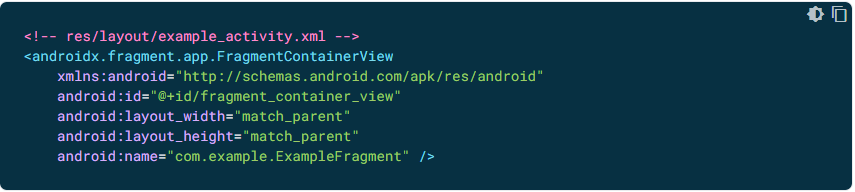
\includegraphics[keepaspectratio, width=12cm]{gambar/fragment_add}
	\caption{Contoh \textit{FragmentContainerView} pada \textit{XML} \citep{developerandroid}}
	\label{gambar:gambar_32}
\end{figure}
	Atribut \textit{android:name} menentukan nama kelas \textit{Fragment} yang akan dibuat \textit{instance}-nya. Saat \textit{layout activity} di-\textit{inflate}, \textit{fragment} yang ditentukan akan dibuat \textit{instance}-nya, \textit{onInflate}() dipanggil pada \textit{fragment} yang baru dibuat \textit{instance}-nya, dan \textit{FragmentTransaction} dibuat untuk menambahkan \textit{fragment} ke \textit{FragmentManager}.
	\item Menambahkan \textit{fragment} secara terprogram
	
	Untuk menambahkan \textit{fragment} secara terprogram ke \textit{layout activity}, \textit{layout} harus menyertakan \textit{FragmentContainerView} yang berfungsi sebahai wadah \textit{fragment}, seperti yang ditunjukkan dalam contoh berikut:
\begin{figure}[H]
	\centering
	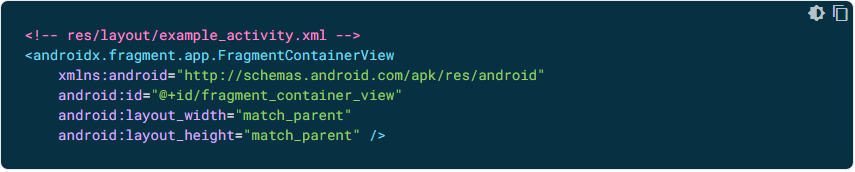
\includegraphics[keepaspectratio, width=12cm]{gambar/fragment_add1}
	\caption{Contoh menambahkan \textit{fragment} secara terprogram. \citep{developerandroid}}
	\label{gambar:gambar_33}
\end{figure}
	Tidak seperti pendekatan \textit{XML}, atribut \textit{android:name} tidak digunakan pada \textit{FragmentContainerView} di sini, jadi tidak ada \textit{fragment} tertentu yang dibuat secara otomatis. Sebagai gantinya, \textit{FragmentTransaction} digunakan untuk membuat \textit{instance fragment} dan menambahkannya ke \textit{layout activity}
	\end{enumerate}
Saat \textit{activity} berjalan, kita dapat melakukan transaksi \textit{fragment} seperti menambahkan, menghapus, atau mengganti \textit{fragment}. Di \textit{FragmentActivity}, kita bisa mendapatkan \textit{instance FragmentManager}, yang dapat digunakan untuk membuat \textit{FragmentTransaction}. Kemudian, kita bisa membuat \textit{instance fragment} dalam metode \textit{onCreate}() \textit{activity} menggunakan \textit{FragmentTransaction.add}(), meneruskan \textit{ID ViewGroup} dari \textit{container} di \textit{layout} dan kelas \textit{fragment} yang ingin ditambahkan, lalu kemudian melakukan transaksi, seperti yang ditunjukkan dalam contoh berikut:
\begin{figure}[H]
	\centering
	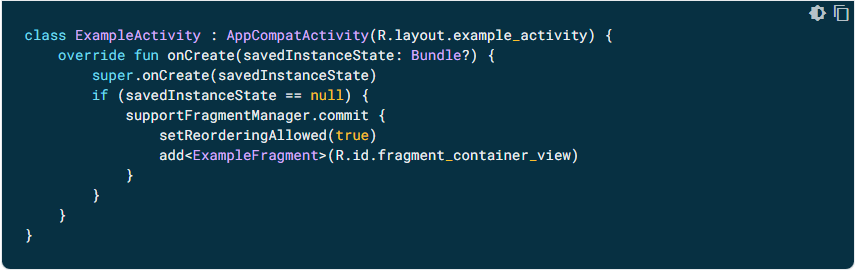
\includegraphics[keepaspectratio, width=12cm]{gambar/fragment_add2}
	\caption{Contoh membuat \textit{FragmentTransaction}. \citep{developerandroid}}
	\label{gambar:gambar_34}
\end{figure}
Pada contoh sebelumnya, perhatikan bahwa transaksi \textit{fragment} hanya dibuat ketika \textit{storedInstanceState} adalah \textit{null}. Ini untuk memastikan bahwa \textit{fragment} hanya ditambahkan sekali, saat \textit{activity} pertama kali dibuat. Saat terjadi perubahan konfigurasi dan \textit{activity} dibuat ualng, \textit{saveInstanceState} tidak lagi \textit{null}, dan \textit{fragment} tidak perlu ditambahkan untuk kedua kalinya, karena \textit{fragment} secara otomatis dipulihkan dari \textit{saveInstanceState}.
Jika \textit{fragment} memerlukan beberapa data awal, argumen dapat diteruskan ke \textit{fragment} dengan menyediakan \textit{bundle} dalam panggilan ke \textit{FragmentTransaction.add}(), seperti yang ditunjukkan di bawah ini:
\begin{figure}[H]
	\centering
	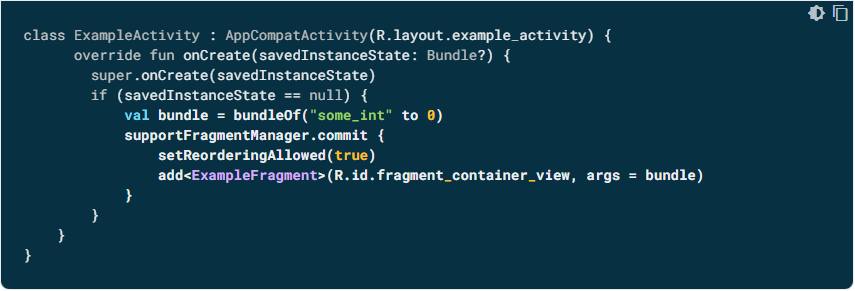
\includegraphics[keepaspectratio, width=12cm]{gambar/fragment_add3}
	\caption{Contoh menambahkan beberapa data awal. \citep{developerandroid}}
	\label{gambar:gambar_35}
\end{figure}
\textit{Bundle} argumen kemudian dapat diambil dari dalam \textit{fragment} dengan memanggil \textit{requireArgument}(), dan metode pengambil \textit{bundle} yang sesuai dapat digunakan untuk mengambil setiap argumen.
\begin{figure}[H]
	\centering
	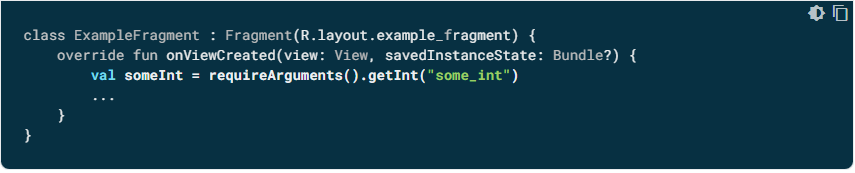
\includegraphics[keepaspectratio, width=12cm]{gambar/fragment_add4}
	\caption{Contoh memanggil \textit{requireArgmunet}(). \citep{developerandroid}}
	\label{gambar:gambar_36}
\end{figure}
\end{enumerate}

\section{\emph{Navigation} dan \emph{menu}}

Navigation mengacu pada interaksi yang memungkinkan pengguna bernavigasi melintasi, masuk, dan mundur dari berbagai bagian konten dalam aplikasi. Komponen navigation dalam Android membantu menerapkan navigasi mulai dari klik tombol sederhana hingga pola yang lebih kompleks, seperti bilah aplikasi dan panel samping navigasi. Komponen navigation juga memastikan pengalaman pengguna yang konsisten dan dapat diprediksi dengan mengikuti serangkaian prinsip yang telah ditetapkan.
Komponen navigation terdiri dari tiga bagian penting:
\begin{enumerate}
\item{\textit{Navigation graph}: sumber daya \textit{XML} yang berisi semua informasi terkait navigasi di satu lokasi terpusat. Ini mencakup semua area konten individual dalam aplikasi, yang disebut \textit{destinations}, serta kemungkinan jalur yang dapat diambil \textit{user} melalui aplikasi.}
\item{\textit{NavHost}: wadah kosong yang menampilkan tujuan dari \textit{navigation graph}. Komponen \textit{navigation} berisi implementasi \textit{default NavHost}, \textit{NavHostFragment}, yang menampilkan tujuan \textit{fragment}.}
\item{\textit{NavController}: objek yang mengelola navigasi aplikasi dalam \textit{NavHost}. \textit{NavController} mengatur pertukaran konten tujuan di \textit{NavHost} saat \textit{user} bergerak di seluruh aplikasi.}
\end{enumerate}

Saat menavigasi melalui aplikasi, kita memberi tahu \textit{NavController} bahwa kita ingin menavigasi di sepanjang jalur tertentu dalam \textit{Navigation graph} atau langsung ke tujuan tertentu. \textit{NavController} kemudian menunjukkan tujuan yang sesuai di \textit{NavHost}. Komponen \textit{navigation} memberikan sejumlah manfaat lain sebagai berikut:

\begin{enumerate}
\item Menangani transaksi fragment.
\item Menangani action up dan action back dengan benar secara default.
\item Menyediakan sumber daya standar untuk animasi dan transisi.
\item Menerapkan dan menangani deep linking.
\item Termasuk pola navigasi UI, seperti panel samping navigasi dan navigasi bawah, dengan sedikit pekerjaan tambahan.
\item Safe Args – plugin Gradle yang menyediakan keamanan jensi saat menavigasi dan meneruskan data antar tujuan.
\item Dukungan ViewModel – kita dapat memasukkan ViewModel ke navigation graph untuk berbagi data terkait UI di antara destination graph.
\item Selain itu juga dapat menggunakan editor navigasi android studio untuk melihat dan mengedit navigation graph.
\end{enumerate}

Cara untuk menggunakan \textit{navigation} adalah sebagai berikut:
\begin{enumerate}
\item \textit{Setup environment}

Untuk menyertakan dukungan \textit{Navigation} dalam proyek, tambahkan dependensi berikut ke file \textit{build.gradle} aplikasi:
\begin{figure}[H]
	\centering
	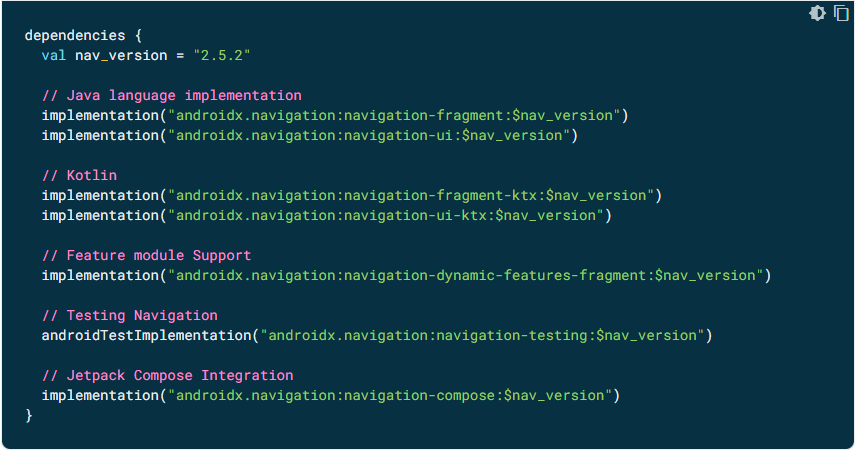
\includegraphics[keepaspectratio, width=12cm]{gambar/navigation_setup}
	\caption{Contoh dependensi untuk \textit{navigation} \citep{developerandroid}}
	\label{gambar:gambar_37}
\end{figure}

\item Buat \emph{navigation graph}

Navigasi terjadi di antara tujuan aplikasi, dimana saja di aplikasi yang dapat dinavigasi oleh pengguna. Tujuan ini terhubung melalui tindakan. \textit{Navigation graph} adalah \textit{file resource} yang berisi semua tujuan dan tindakan. \textit{Graph} mewakili semua jalur \textit{navigation} aplikasi.

Gambar 1 menunjukkan representasi visual \textit{graph navigation} untuk aplikasi sampel yang berisi enam tujuan yang dihubungkan oleh lima tindakan. Setiap tujuan diwakili oleh gambar mini pratinjau, dan tindakan menghubungkan diwakili oleh panah yang menunjukkan bagaimana pengguna dapat menavigasi dari satu tujuan ke tujuan lainnya.
\begin{figure}[H]
	\centering
	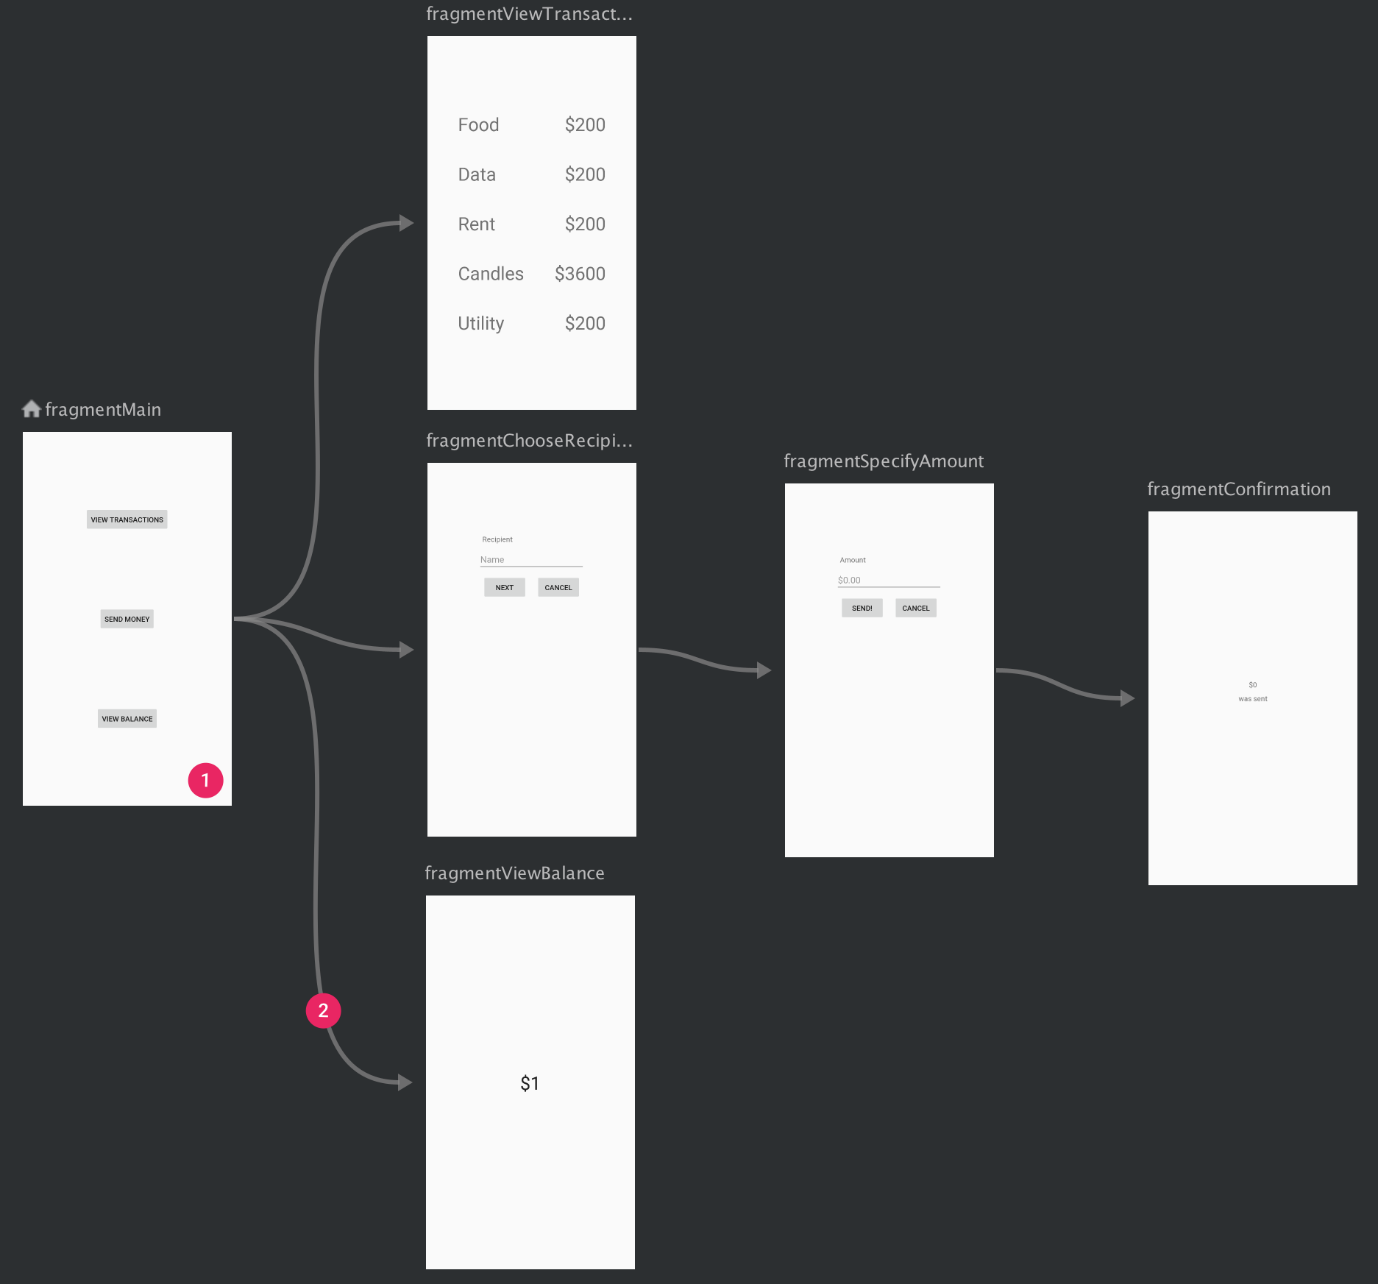
\includegraphics[keepaspectratio, width=12cm]{gambar/navigation_graph1}
	\caption{Grafik navigasi yang menampilkan pratinjau dari enam tujuan berbeda yang terhubung melalui lima tindakan \citep{developerandroid}}
	\label{gambar:gambar_38}
\end{figure}

	\begin{enumerate}
	\item \textit{Destinations} adalah area konten yang berbeda di aplikasi.
	\item \textit{Actions} adalah koneksi logis antara tujuan yang mewakili jalur yang dapat diambil pengguna.
	\end{enumerate}
	
Untuk menambahkan \textit{graph navigation} ke proyek adalah sebagai berikut:
	\begin{enumerate}
	\item Di jendela \textit{project}, klik kanan pada direktori \textit{res} dan pilih \textit{New} > \textit{Android Resource File}. Dialog \textit{file resource} baru muncul.
	\item Ketik nama di \textit{field} nama \textit{file}, seperti \textit{$"nav_graph"$}.
	\item Pilih navigasi dari daftar \textit{drop-down} jenis \textit{resource}, lalu klik \textit{Ok}.
	\end{enumerate}
	
Ketika menambahkan \textit{graph navigation} pertama, \textit{Android Studio} membuat direktori \textit{resource navigation} di dalam direktori \textit{res}. Direktori ini berisi \textit{file resource graph navigation} (\textit{$nav_graph.xml$}, misalnya).

\item \emph{Navigation editor}

Setelah menambahkan \textit{graph}, \textit{Android Studio} membuka \textit{frap} di \textit{Navigation Editor}. Di sini dapat mengedit \textit{navigation graph} secara visual atau langsung mengedit \textit{XML} yang mendasarinya.
\begin{figure}[H]
	\centering
	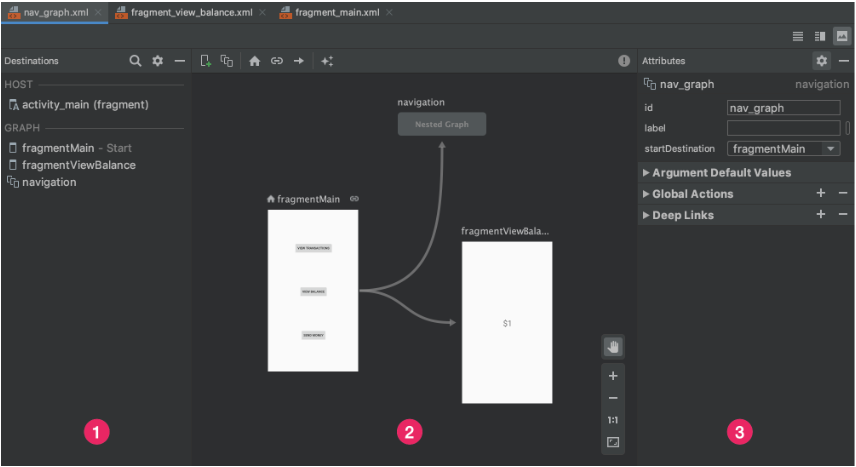
\includegraphics[keepaspectratio, width=12cm]{gambar/navigation_graph2}
	\caption{\textit{Navigation Editor} \citep{developerandroid}}
	\label{gambar:gambar_39}
\end{figure}

	\begin{enumerate}
	\item \textit{Destinations panel}: mencantumkan \textit{host} navigasi dan semua tujuan yang saat ini ada di \textit{Graph Editor}.
	\item 	\textit{Graph Editor}: berisi representasi visual dari \textit{navigation graph}. Dapat beralih antara tampilan desain dan representasi \textit{XML} yang mendasarinya dalam tampilan teks.
	\item \textit{Attributes}: menampilkan atribut untuk item yang saat ini dipilih dalam \textit{navigation graph}.
	\end{enumerate}
	
Klik tab \textit{Text} untuk melihat \textit{XML} yang sesuai, yang akan terlihat mirip dengan gambar berikut:
\begin{figure}[H]
	\centering
	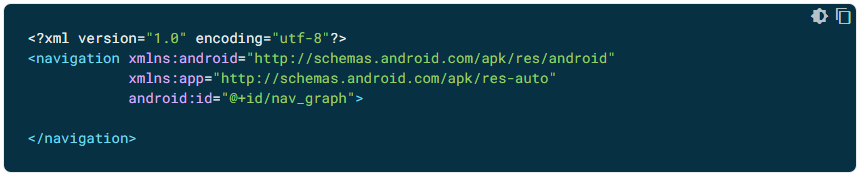
\includegraphics[keepaspectratio, width=12cm]{gambar/navigation_graph3}
	\caption{Contoh \textit{XML navigation graph} \citep{developerandroid}}
	\label{gambar:gambar_40}
\end{figure}

Elemen <\textit{navigation}> adalah elemen \textit{root} dari \textit{navigation graph}. Saat menambahkan tujuan dan menghubungkan tindakan ke \textit{graph}, dapat melihat elemen <\textit{destination}> dan <\textit{action}> yang sesuai di sini sebagai elemen turunan. Jika memiliki \textit{nest graph}, \textit{graph} tersebut muncul sebagai elemen anak <\textit{navigation}>.

\item \emph{Menu}

\textit{Menu} adalah komponen \textit{user interface} yang umum di banyak jenis aplikasi. Untuk memberikan pengalaman pengguna yang familiar dan konsisten harus menggunakan \textit{menu API} untuk menyajikan \textit{user action} dan opsi lain dalam \textit{activity}.

Mulai \textit{android} 3.0, perangkat yang diberdayakan android tidak lagi diharuskan menyediakan tombol \textit{menu} khusus. Dengan perubahan ini, aplikasi android harus bermigrasi dari ketergantungan pada panel menu 6 item tradisional dan sebagai gantinya menyediakan bilah aplikasi untuk menyajikan tindakan pengguna yang umum.

Meskipun desan dan pengalaman pengguna untuk beberapa \textit{item menu} telah berubah, semantik untuk menentukan serangkaian tindakan dan opsi masih didasarkan pada \textit{menu API}. Cara membuat tiga tipe dasar \textit{menu}: \textit{Options menu and app bar}, \textit{Context menu and contextual action mode}, \textit{Popup menu}.

Untuk semua jenis \textit{menu}, Android menyediakan format \textit{XML} standar untuk mendefinisikan \textit{item menu}. Alih-alih membuat \textit{menu} dalam kode \textit{aktivitas}, kita harus mendefinisikan \textit{menu} dan semua itemnya dalam sumber data \textit{menu XML}. Anda kemudian dapat mengembang sumber daya menu (memuatnya sebagai objek Menu) di \textit{activity} atau \textit{fragment}.

Menggunakan menu resource adalah praktik yang baik karena beberapa alasan:
	\begin{enumerate}
	\item Lebih mudah untuk memvisualisasikan struktur \textit{menu} dalam \textit{XML}.
	\item Ini memisahkan konten untuk \textit{menu} dari \textit{applications behavioral code}.
	\item Ini memungkinkan membuat konfigurasi \textit{menu} alternatif untuk berbagai versi platform, ukuran layar, dan konfigurasi lainnya dengan memanfaatkan \textit{framework} aplikasi.
	\end{enumerate}

Untuk menentukan menu, buat file XML di dalam direktori res/menu/ dan buat menu dengan elemen berikut:
	\begin{enumerate}
	\item 1.	<\textit{menu}> = Mendefinisikan menu, yang merupakan wadah untuk \textit{item menu}. Elemen <\textit{menu}> harus menjadi simpul akar untuk \textit{file} dan dapat menampung satu atau lebih elemen <\textit{item}> dan <\textit{group}>.
	\item <\textit{item}> = Membuat \textit{menu item}, yang mewakili satu \textit{item} dalam \textit{menu}. Elemen ini mungkin berisi elemen sarang <\textit{menu}> yang membuat \textit{submenu}.
	\item <\textit{group}> = Wadah opsional yang tidak terlihat untuk elemen <\textit{item}>. Ini memungkinkan untuk mengkategorikan \textit{item menu} sehingga mereka berbagi properti seperti status aktif dan visibilitas.
	\end{enumerate}

Berikut contoh menu bernama $game_menu.xml$:
\begin{figure}[H]
	\centering
	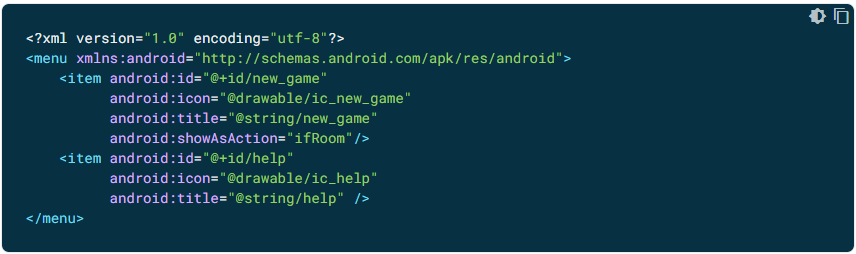
\includegraphics[keepaspectratio, width=12cm]{gambar/menu}
	\caption{Contoh \textit{menu} \citep{developerandroid}}
	\label{gambar:gambar_41}
\end{figure}

Elemen <\textit{item}> mendukung beberapa atribut yang dapat digunakan untuk menentukan tampilan dan perilaku item. \textit{Item} dalam \textit{menu} di atas mencakup atribut berikut:
	\begin{enumerate}
	\item \textit{android:id} = \textit{ID resource} yang unik untuk \textit{item}, yang memungkinkan aplikasi mengenali \textit{item} saat pengguna memilihnya.
	\item \textit{android:icon} = Referensi ke \textit{resource} gambar untuk digunakan sebagai ikon \textit{item}.
	\item \textit{android:title} = referensi ke \textit{string} untuk digunakan sebagai judul \textit{item}.
	\item \textit{android:showAsAction} = Menentukan kapan dan bagaimana \textit{item} ini akan muncul sebagai \textit{item} tindakan di bilah aplikasi.
	\end{enumerate}
Ini adalah atribut terpenting yang harus digunakan, tetapi masih banyak lagi yang tersedia.
\end{enumerate}

\section{Layouting}

Layout mendefinisikan struktur untuk user interface di aplikasi, seperti dalam suatu aktivitas. Semua elemen dalam layout dibangun menggunakan hierarki objek View dan ViewGroup. View biasanya menggambar sesuatu yang dapat dilihat dan berinteraksi dengan pengguna. Sedangkan ViewGroup adalah wadah tak terlihat yang mendefinisikan struktur layout untuk View dan objek ViewGroup lainnya.
\begin{figure}[H]
	\centering
	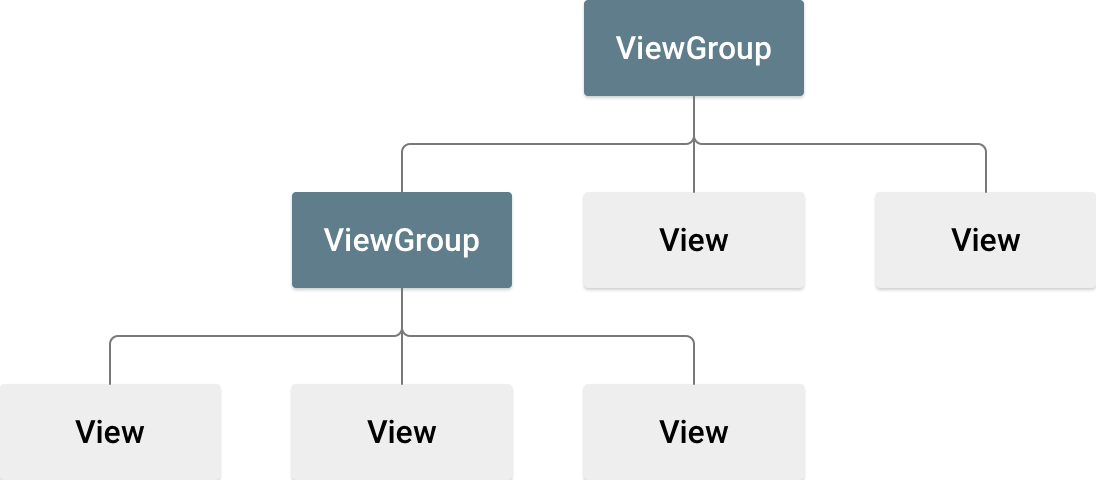
\includegraphics[keepaspectratio, width=12cm]{gambar/layout_hirarki}
	\caption{Ilustrasi hierarki tampilan, yang menentukan tata letak UI \citep{developerandroid}}
	\label{gambar:gambar_42}
\end{figure}

Objek \textit{View} biasanya disebut "\textit{widget}" dan bisa menjadi salah satu dari banyak \textit{subclass}, seperti \textit{Button} atau \textit{TextView}. Objek \textit{ViewGroup} biasanya disebut "\textit{layout}" dapat menjadi salah satu dari banyak jenis yang menyediakan struktur \textit{layout} yang berbeda, seperti \textit{LinearLayout} atau \textit{ConstraintLayout}. Deklarasi \textit{layout} dapat dengan dua cara:
\begin{enumerate}
\item Deklarasikan elemen UI dalam \textit{XML}. 

Android menyediakan kosakata \textit{XML} langsung yang sesuai dengan kelas dan subkelas \textit{View}, seperti untuk \textit{widget} dan \textit{layout}. Kita juga dapat menggunakan \textit{layout} editor android studio untuk membangun \textit{layout XML} menggunakan \textit{interface} \textit{“drag-and-drop”}.
\item Buat \textit{instance} elemen \textit{layout} saat \textit{runtime}. 

Aplikasi kita dapat membuat objek \textit{View} dan \textit{ViewGroup} (dan memanipulasi propertinya) secara terprogram.
\end{enumerate}

Mendeklarasikan UI dalam \textit{XML} memungkinkan kita untuk memisahkan presentasi aplikasi dari kode yang mengontrol perilakunya. Menggunakan file \textit{XML} juga memudahkan untuk menyediakan \textit{layout} yang berbeda untuk ukuran dan orientasi layar yang berbeda.
Kerangka kerja android memberi kita fleksibilitas untuk menggunakan salah satu atau kedua metode ini untuk membangun UI aplikasi. Misalnya bisa mendeklarasikan \textit{layout default} aplikasi dalam \textit{XML}, lalu memodifikasi \textit{layout} saat waktu proses.

Dengan menggunakan kosakata \textit{XML} Android, kita dapat dengan cepat mendesain tata letak UI dan elemen layar yang dikandungnya dengan cara yang sama seperti membuat halaman web dalam \textit{HTML} dengan serangkaian elemen bersarang.

Setiap \textit{file layout} harus berisi tepat satu elemen \textit{root} yang harus berupa objek \textit{View} atau \textit{ViewGroup}. Setelah menentukan elemen \textit{root}, dapat menambahkan objek atau \textit{widget layout} tambahan sebagai elemen turunan untuk membangun hierarki \textit{View} yang mendefinisikan \textit{layout} secara bertahap. Contohnya ini \textit{layout XML} yang menggunakan \textit{LinearLayout} vertikal untuk menampung \textit{TextView} dan \textit{Button}:
\begin{figure}[H]
	\centering
	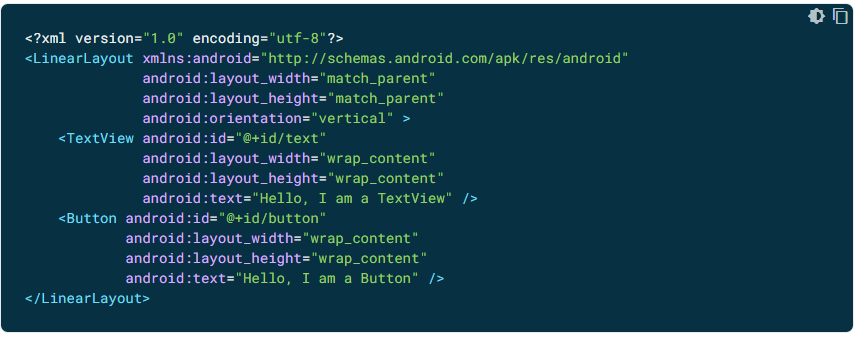
\includegraphics[keepaspectratio, width=12cm]{gambar/layout_linearlayout}
	\caption{Contoh \textit{layout XML} yang menggunakan \textit{LinearLayout} \citep{developerandroid}}
	\label{gambar:gambar_43}
\end{figure}

Setelah dideklarasikan \textit{layout} dalam \textit{XML}, simpan file dengan ekstensi \textit{.xml} di direktori \textit{res/layout/} proyek Android kita sehingga akan dikompilasi dengan benar.

Saat mengompilasi aplikasi, setiap \textit{file layout XML} dikompilasi ke dalam \textit{resource View}. Diharuskan memuat \textit{resource layout} dari kode aplikasi, dalam implementasi \textit{callback Activity.onCreate}(). Lakukan dengan memanggil \textit{setContentView}(), meneruskannya referensi ke \textit{resource layout} dalam bentuk: R\textit{$.layout.layout_file_name$}. Misalnya, jika \textit{layout XML} disimpan sebagai \textit{$main_layout.xml$}, maka akan memuatnya untuk \textit{activity} seperti berikut:
\begin{figure}[H]
	\centering
	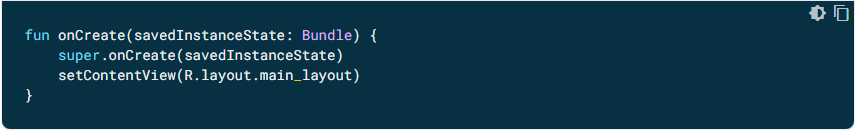
\includegraphics[keepaspectratio, width=12cm]{gambar/layout_setcontentview}
	\caption{Contoh menggunakan \textit{setContentView}() \citep{developerandroid}}
	\label{gambar:gambar_44}
\end{figure}
Metode \textit{callback onCreate}() dalam \textit{activity} dipanggil oleh \textit{framework} Android saat \textit{activity} diluncurkan.
Setiap objek \textit{View} dan \textit{ViewGroup} mendukung berbagai atribut \textit{XML} mereka sendiri. Beberapa atribut khusus untuk objek \textit{View} (misalnya, \textit{TextView} mendukung atribut \textit{textSize}), tetapi atribut ini juga diwarisi oleh objek \textit{View} apa pun yang dapat memperluas kelas ini. Beberapa umum untuk semua objek \textit{View}, karena mereka diwarisi dari kelas \textit{View root} (seperti atribut \textit{id}). Dan, atribut lainnya dianggap sebagai "\textit{parameter layout}", yang merupakan atribut yang menjelaskan orientasi \textit{layout} tertentu dari objek \textit{View}, seperti yang didefinisikan oleh objek induk \textit{ViewGroup} objek tersebut.
Objek \textit{View} apa pun mungkin memiliki \textit{ID integer} yang terkait dengannya, untuk mengidentifikasi \textit{View} secara unik di dalam hierarki. Saat aplikasi dikompilasi, \textit{ID} ini direferensikan sebagai bilangan bulat, tetapi \textit{ID} biasanya ditetapkan dalam \textit{file XML layout} sebagai \textit{string}, dalam atribut \textit{id}. Ini adalah atribut \textit{XML} yang umum untuk semua objek \textit{View} (didefinisikan oleh kelas \textit{View}) dan akan sering digunakan. Sintaks untuk \textit{ID} di dalam \textit{tag XML} adalah:
\begin{figure}[H]
	\centering
	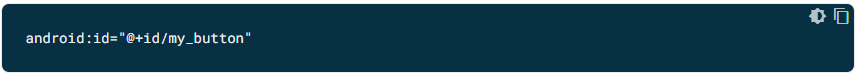
\includegraphics[keepaspectratio, width=12cm]{gambar/layout_tagidbutton}
	\caption{Contoh sintaks untuk \textit{tag ID} \citep{developerandroid}}
	\label{gambar:gambar_45}
\end{figure}
Simbol \textit{(@)} di awal \textit{string} menunjukkan bahwa parser \textit{XML} harus mengurai dan memperluas sisa \textit{string ID} dan mengidentifikasinya sebagai \textit{resource ID}. Tanda tambah (+) berarti bahwa ini adalah nama \textit{resource} baru yang harus dibuat dan ditambahkan ke \textit{resource} kita (dalam \textit{file R.java}). Ada sejumlah \textit{resource ID} lain yang ditawarkan oleh \textit{framework} Android. Saat mereferensikan \textit{ID resource} Android, kita tidak memerlukan simbol tambah, tetapi harus menambahkan \textit{namespace package} Android, seperti:
\begin{figure}[H]
	\centering
	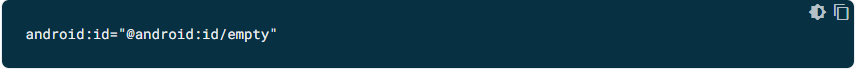
\includegraphics[keepaspectratio, width=12cm]{gambar/layout_tagidbutton2}
	\caption{Contoh menggunakan \textit{namespace package} Android \citep{developerandroid}}
	\label{gambar:gambar_46}
\end{figure}
Dengan \textit{namespace package} Android di tempat, kita sekarang mereferensikan \textit{ID} dari kelas \textit{resource android.R}, bukan dari kelas \textit{resource} lokal.
Untuk membuat View dan mereferensikannya dari aplikasi, pola umumnya adalah:
\begin{enumerate}
\item Tentukan \textit{View}/ \textit{widget} dalam \textit{file layout} dan tetapkan \textit{ID} unik
\begin{figure}[H]
	\centering
	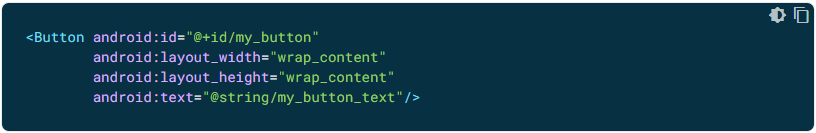
\includegraphics[keepaspectratio, width=12cm]{gambar/layout_view1}
	\caption{Menetapkan \textit{ID} unik \citep{developerandroid}}
	\label{gambar:gambar_47}
\end{figure}
\item Kemudian buat \textit{instance} objek \textit{view} dan ambil dari \textit{layout} (biasanya dalam metode \textit{onCreate}())
\begin{figure}[H]
	\centering
	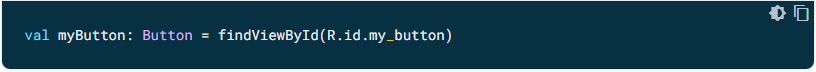
\includegraphics[keepaspectratio, width=12cm]{gambar/layout_view2}
	\caption{Membuat \textit{instance} objek \textit{view} \citep{developerandroid}}
	\label{gambar:gambar_48}
\end{figure}
\end{enumerate}
Mendefinisikan \textit{ID} untuk objek \textit{view} penting saat membuat \textit{RelativeLayout}. Dalam \textit{RelativeLayout}, \textit{view} dapat menentukan \textit{layout}nya relatif terhadap tampilan \textit{view} lainya, yang direferensikan oleh \textit{ID} unik. \textit{ID} tidak harus unik diseluruh \textit{tree}, tetapi harus unik di dalam bagian pohon yang dicari (yang mungkin sering berupa seluruh \textit{tree}, jadi sebaiknya benar-benar unik jika memungkinkan).

\section{\emph{Retrofit}}

\begin{enumerate}
\item Pengenalan

Cara menggunakan \textit{retrofit} dalam Android dengan contoh API \textit{GithubService}:

	\begin{enumerate}
	\item \textit{Retrofit} mengubah API HTTP menjadi \textit{interface} Java.
	\begin{figure}[H]
		\centering
		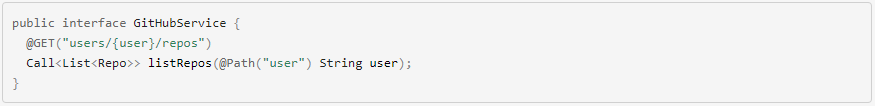
\includegraphics[keepaspectratio, width=12cm]{gambar/retrofit1}
		\caption{Contoh \textit{retrofit} mengubah API menjadi \textit{interface} \citep{retrofit2023}}
		\label{gambar:gambar_49}
	\end{figure}
	
	\item Kelas \textit{Retrofit} menghasilkan implementasi \textit{interface GitHubService}.
	\begin{figure}[H]
		\centering
		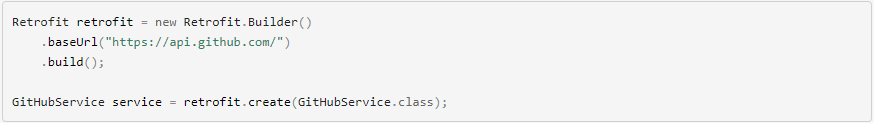
\includegraphics[keepaspectratio, width=12cm]{gambar/retrofit2}
		\caption{Kelas \textit{retrofit} \citep{retrofit2023}}
		\label{gambar:gambar_50}
	\end{figure}
	
	\item Setiap \textit{Call} dari \textit{GitHubService} yang dibuat dapat membuat \textit{request} HTTP sinkron atau asinkron ke server web jarak jauh.
	\begin{figure}[H]
		\centering
		
\includegraphics[keepaspectratio, width=12cm]{gambar/retrofit3}
		\caption{\textit{Call} \citep{retrofit2023}}
		\label{gambar:gambar_51}
	\end{figure}
	\end{enumerate}

Menggunakan anotasi untuk menjelaskan request HTTP:
	\begin{enumerate}
		\item Penggantian parameter URL dan dukungan parameter kueri
		\item Konversi objek ke request body (misalnya JSON, protocol buffers)
		\item Multi-bagian request body dan unggahan file
	\end{enumerate}
	
\item Deklarasi API

Anotasi pada metode interface dan parameternya menunjukkan bagaimana request akan ditangani.
	\begin{enumerate}
	\item \emph{Request method}
	
	Setiap metode harus memiliki anotasi HTTP yang menyediakan metode request dan URL relatif. Ada delapan anotasi bawaan: HTTP, GET, POST, PUT, PATCH, DELETE, OPTIONS, dan HEAD. URL relatif resource ditentukan dalam anotasi.
	\begin{figure}[H]
		\centering
		
\includegraphics[keepaspectratio, width=12cm]{gambar/retrofit4}
		\caption{Contoh request GET \citep{retrofit2023}}
		\label{gambar:gambar_52}
	\end{figure}
	
	Dapat juga menentukan parameter kueri di URL
	\begin{figure}[H]
		\centering
		
\includegraphics[keepaspectratio, width=12cm]{gambar/retrofit5}
		\caption{Contoh request GET dengan menentukan parameter kueri di URL \citep{retrofit2023}}
		\label{gambar:gambar_53}
	\end{figure}
	
	\item Manipulasi URL
	
	Request URL dapat diperbarui secara dinamis menggunakan blok dan parameter pengganti pada metode. Blok pengganti adalah string alfanumerik yang dikelilingi oleh { dan }. Parameter yang sesuai harus dianotasi dengan @Path menggunakan string yang sama.
	\begin{figure}[H]
		\centering
		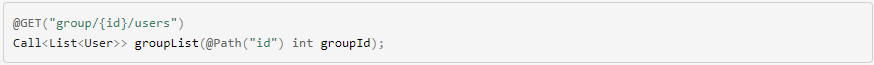
\includegraphics[keepaspectratio, width=12cm]{gambar/retrofit6}
		\caption{Contoh request URL secara dinamis \citep{retrofit2023}}
		\label{gambar:gambar_54}
	\end{figure}
	
	Parameter kueri juga dapat ditambahkan.
	\begin{figure}[H]
		\centering
		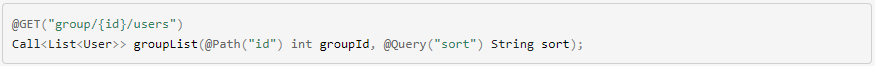
\includegraphics[keepaspectratio, width=12cm]{gambar/retrofit7}
		\caption{Contoh parameter kueri ditambahkan \citep{retrofit2023}}
		\label{gambar:gambar_55}
	\end{figure}
	
	Untuk kombinasi parameter kueri yang kompleks, Map dapat digunakan.
	\begin{figure}[H]
		\centering
		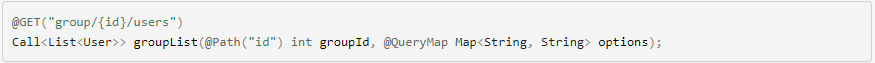
\includegraphics[keepaspectratio, width=12cm]{gambar/retrofit8}
		\caption{Contoh menggunakan Map \citep{retrofit2023}}
		\label{gambar:gambar_56}
	\end{figure}
	
	\item \emph{Request Body}
	
	Sebuah objek dapat ditentukan untuk digunakan sebagai body request HTTP dengan anotasi @Body.
	\begin{figure}[H]
		\centering
		
\includegraphics[keepaspectratio, width=12cm]{gambar/retrofit9}
		\caption{Contoh anotasi Body \citep{retrofit2023}}
		\label{gambar:gambar_57}
	\end{figure}
	
	Objek juga akan dikonversi menggunakan konverter yang ditentukan pada instance Retrofit. Jika tidak ada konverter yang ditambahkan, hanya RequestBody yang dapat digunakan.
	
	\item Formulir dikode dan multipart
	
	Metode juga dapat dideklarasikan untuk mengirim data yang disandikan bentuk dan multibagian. Data yang disandikan formulir dikirim ketika @FormUrlEncoded ada di metode. Setiap pasangan nilai kunci dianotasi dengan @Field yang berisi nama dan objek yang memberikan nilai.
	\begin{figure}[H]
		\centering
		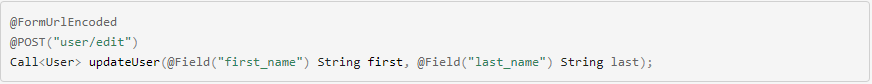
\includegraphics[keepaspectratio, width=12cm]{gambar/retrofit10}
		\caption{Contoh dikode \citep{retrofit2023}}
		\label{gambar:gambar_58}
	\end{figure}
	
	Request multipart digunakan ketika @Multipart hadir pada metode. Bagian dideklarasikan menggunakan anotasi @Part.
	\begin{figure}[H]
		\centering
		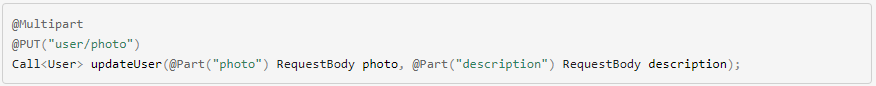
\includegraphics[keepaspectratio, width=12cm]{gambar/retrofit11}
		\caption{Contoh multipart \citep{retrofit2023}}
		\label{gambar:gambar_59}
	\end{figure}
	
	Bagian multipart menggunaakn salah satu konverter Retrofit atau mereka dapat mengimplementasikan RequestBody untuk menangani serialisasi mereka sendiri.
	
	\item Manipulasi \emph{header}
	
	Kita dapat mengatur tajuk statis untuk suatu metode menggunakan anotasi @Headers.
	\begin{figure}[H]
		\centering
		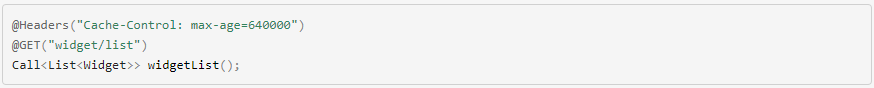
\includegraphics[keepaspectratio, width=12cm]{gambar/retrofit12}
		\caption{Contoh anotasi header \citep{retrofit2023}}
		\label{gambar:gambar_60}
	\end{figure}
	
	\begin{figure}[H]
		\centering
		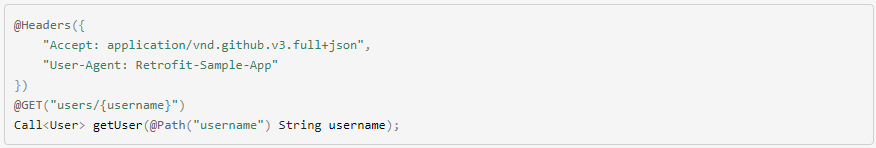
\includegraphics[keepaspectratio, width=12cm]{gambar/retrofit13}
		\caption{Contoh anotasi header \citep{retrofit2023}}
		\label{gambar:gambar_61}
	\end{figure}
	
	Perhatikan bahwa header tidak saling menimpa. Semua header dengan nama yang sama akan disertakan dalam request.
	Requset header dapat diperbarui secara dinamis menggunakan anotasi @Header. Parameter yang sesuai harus diberikan ke @Header. Jika nilainya null, header akan dihilangkan. Jika tidak, toString akan dipanggil pada nilai, dan hasilnya digunakan.
	\begin{figure}[H]
		\centering
		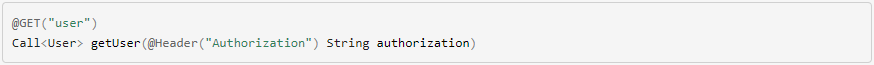
\includegraphics[keepaspectratio, width=12cm]{gambar/retrofit14}
		\caption{Contoh header dinamis \citep{retrofit2023}}
		\label{gambar:gambar_62}
	\end{figure}
	
	Mirip dengan parameter kueri, untuk kombinasi tajuk yang kompleks, Map dapat digunakan.
	\begin{figure}[H]
		\centering
		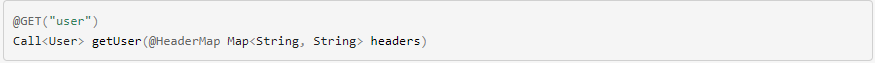
\includegraphics[keepaspectratio, width=12cm]{gambar/retrofit15}
		\caption{Contoh header kompleks menggunakan Map \citep{retrofit2023}}
		\label{gambar:gambar_63}
	\end{figure}
	
	Header yang perlu ditambahkan ke setiap request dapat ditentukan menggunakan interseptor OkHttp.
	\end{enumerate}
	
\item Konfigurasi retrofit

Retrofit adalah kelas yang digunakan untuk mengubah interface API menjadi objek yang dapat dipanggil. Secara default, Retrofit akan memberi standar yang normal untuk platform tetapi memungkinkan untuk penyesuaian.

	\begin{enumerate}
	\item Converters
	
	Secara default, Retrofit hanya dapat melakukan deserialize body HTTP ke dalam tipe ResponseBody OkHttp dan hanya dapat meneripa tipe RequestBody untuk @Body. Konverter dapat ditambahkan untuk mendukung jenis lain. Enam modul bersaudara mengadaptasi pustaka serialisasi populer untuk kenyamanan pengguna.
		\begin{enumerate}
		\item Gson: com.squareup.retrofit2:converter-gson
		\item Jackson: com.squareup.retrofit2:converter-jackson
		\item Moshi: com.squareup.retrofit2:converter-moshi
		\item Protobuf: com.squareup.retrofit2:converter-protobuf
		\item Wire: com.squareup.retrofit2:converter-wire
		\item Simple XML: com.squareup.retrofit2:converter-simplexml
		\item JAXB: com.squareup.retrofit2:converter-jaxb
		\item Scalars (primitives, boxed, dan String): com.squareup.retrofit2:converter-scalars
		\end{enumerate}
		
	Berikut adalah contoh penggunaan kelas GsonConverterFactory untuk menghasilkan implementasi interface GitHubService yang menggunakan Gson untuk deserialisasinya.
	\begin{figure}[H]
		\centering
		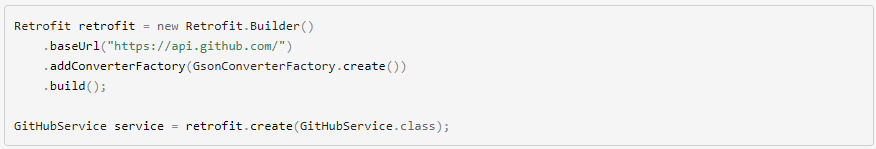
\includegraphics[keepaspectratio, width=12cm]{gambar/retrofit16}
		\caption{Contoh kelas GsonConverterFactory \citep{developerandroid}}
		\label{gambar:gambar_64}
	\end{figure}
	
	\item Custom Converters
	
	Jika perlu berkomunikasi dengan API yang menggunakan format konten yang tidak didukung Retrofit secara langsung (misalnya YAML, txt, format kustom) atau ingin menggunakan pustakan lain untuk mengimplementasikan format yang sudah ada, pengguna dapat dengan mudah membuat konverter pengguna sendiri. Buat kelas yang memperluas kelas Converter.Factory dan berikan instance saat membuat adaptor pengguna.
	\end{enumerate}

\item Download retrofit

Kode sumber Retrofit, sampelnya, dan situs web resmi tersedia di GitHub. Lalu pada Gradle tambahkan:
\begin{figure}[H]
	\centering
	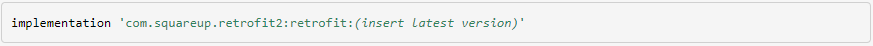
\includegraphics[keepaspectratio, width=12cm]{gambar/retrofit17}
	\caption{Contoh mendownload retrofit pada Gradle \citep{developerandroid}}
	\label{gambar:gambar_65}
\end{figure}

Retrofit membutuhkan minimal Java 8+ atau Android API 21+.
\end{enumerate}

\section{Manajemen Keperawatan}
\begin{enumerate}
\item \textit{Medical Record}

Sebelum dilakukannya proses penyembuhan oleh perawat, pasien diharuskan untuk mengisi data-data terkait diri mereka. Data-data tersebut diperlukan dalam meningkatkan keberhasilan penyembuhan sang pasien. Salah satu data yang diperlukan dalam proses penyembuhan yaitu rekap kunjungan pasien.

\item Rekap kunjungan pasien

Hal ini untuk mencatat tanggal kunjungan, jumlah kunjungan, perawat yang mengobati, dan hasil dari pemeriksaan serta keterangan yang diperlukan untuk membantu proses penyembuhan di hari kunjungan berikutnya.

\item Surat pernyataan persetujuan tindakan

Selanjutnya yaitu surat pernyataan persetujuan dari pasien. Pihak rumah sakit atau klinik meminta agar pasien menandatangani surat pernyataan persetujuan tindakan ini untuk dapat leluasa dalam melakukan perawatan. Pasien diberikan informasi mengenai kondisi pasien tersebut dan diharap mengerti serta memahami konsekuensi dari tindakan yang akan dilakukan sesuai dengan penjelasan yang telah diberikan oleh tenaga kesehatan yang melakukan perawatan.

\item Status pasien

Status pasien ini berisi data-data pribadi pasien tersebut. Status pasien terdiri dari nomor registrasi, nama lengkap pasien, agama/keyakinan pasien, tempat, tanggal lahir dan usia pasien, jenis kelamin pasien, alamat dan nomor telepon rumah pasien, nomor \textit{handphone} dan alamat email pasien, diagnosa keperawatan saat ini, \textit{therapist} utama, tim \textit{therapist}, dan alergi yang dialami oleh pasien.

\item Pengkajian umum luka

Pada pengkajian umum luka ini meliputi riwayat kejadian luka, riwayat perawatan sebelumnya dan faktor-faktor penyulit proses penyembuhan luka pada pasien.

\item Pengkajian lokal luka

Perawat melakukan pemeriksaan pada pasien yang nantinya akan menjadi penunjang keberhasilan penyembuhan luka pasien. Pemeriksaan yang dilakukan oleh perawat ialah tipe luka, tipe penyembuhan, gambar luka, pemeriksaan tanda-tanda vital dan penunjang, serta pemeriksaan fisik dan penunjang lainnya.
Dilanjutkan dengan skoring luka yang dilakukan oleh perawat menggunakan assessment tools yang sudah disiapkan. Dalam gambar ini saya mengambil contoh skoring luka berdasarkan klinik moist care pusat penyembuhan luka.

\item Catatan perkembangan

Diakhir pemeriksaan pengkajian luka, perawat atau therapist memberi kesimpulan tujuan keperawatan yang nantinya dijadikan evaluasi dan rencana tindakan atau intervensi selanjutnya pada pasien.

\item Standar kompetensi perawat dalam perawatan luka

\textit{Enterostomal Therapy Nurse} atau ETN merupakan spesialisasi keperawatan dalam bidang \textit{enterostomal therapy}, \textit{“expert”} dalam melakukan asuhan keperawatan \textit{stoma}, perawatan luka dan \textit{inkontinensia}. Atau yang dikenal dengan nama lainnya adalah \textit{Wound Stoma and Continence Nurse Specialist} atau WOCNS. Pertama kalinya \textit{“Enterostomal Therapist”} dikenalkan oleh Dr. Rupert Turnbull, dari \textit{Cleveland clinic}, USA pada tahun 1958. Beliau bersama dengan salah satu pasien ileostominya, Mrs. Norma Gill, mengadakan program pelatihan untuk para profesional pertama kali tentang bagaimana membantu pasien stoma dalam menjalani kehidupannya yang baru.

Sejak pelatihan pertama di \textit{Cleveland clinic}, USA, tanggung jawab keilmuan \textit{Enterostomal Therapist} semakin berkembang, kemudian berdirilah sekolah perawatan \textit{Enterostomal Therapist} dibawah \textit{World Council of Enterostomal Therapist}(WCET) atau yang dikenal dengan ETNEP(\textit{Enterostomal Therapy Nurse Education Programme}).
Di akhir tahun 1970, \textit{Enterostomal Therapist} mengembangkan diri pada bidang spesialisasi managemen perawatan luka kronik. Awalnya adalah karena keberhasilan dalam merawat komplikasi kulit disekitar stoma. Saat ini, hampir sebagian team \textit{Enterostomal Therapist} melakukan perawatan luka kronik yang meliputi \textit{pressure ulcer}, \textit{dehisensi} luka operasi, \textit{fistula}, \textit{malignant wound}, \textit{vascular ulcer} dan luka diabetikum.

ETN dalam wadah WCET (\textit{World Council of Enterostomal Therapists}) sebagai lembaga non profit internasional telah mengembangkan sayapnya diseluruh penjuru eropa, america dan asia pasific. Keberadaan organisasi ini telah diakui secara international sebagai profesi keperawatan yang profesional. Pengembangan profesi dilakukan dengan mengadakan kongres 2 tahunan dan ETNEP. Di lima tahun terakhir ini, WCET telah membuka diri dengan konsep \textit{twinning} program edukasi untuk lebih memperluas bidang keilmuan \textit{enterostomal therapy nurse} terutama di asia, untuk mempermudah adanya kesulitan dalam bahasa.

Peran ETN adalah untuk memberikan perawatan secara langsung dan konseling pada ostomate selama berada di RS dan di rumah. Memfasilitasi rehabilitasi bagi ostomate untuk berhubungan dengan dokter, ahli gizi atau \textit{sosial worker}. Merancang program edukasi bagi ostomate dan keluarganya dalam bentuk grup/ kelompok. Berpartisipasi dalam pendidikan keperawatan dalam hal pembelajaran tentang perawatan ostomi, \textit{wound} dan \textit{inkontinensia} Melakukan uji coba produk dan melakukan penelitian yang berhubungan dengan pemakaiannya untuk meningkatkan kualitas pelayanan. Melakukan pencatatan data, statistik dan yang berhubungan dengan pelayanan \textit{Enterostomal Therapy}.

Di Indonesia, organisasi yang resmi menyelenggarakan pendidikan ETNEP dari WCET adalah InWOCNA (\textit{Indonesia Wound Ostomy Continence Nurse Association}). Dengan mengikuti ETNEP, perawat dapat sertifikat keahlian resmi dari InWOCNA dan sudah diakui oleh PPNI (Persatuan Perawat Nasional Indonesia) bahwa perawat tersebut telah mengikuti pelatihan sesuai dengan kurikulum InWOCNA. \citep{inwocna}

\end{enumerate}
\begin{figure}[H]
	\centering
	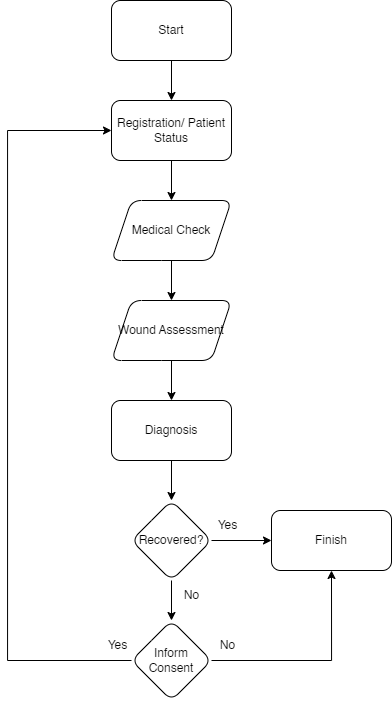
\includegraphics[keepaspectratio, width=8cm]{gambar/flowchart_manajemen_perawatan_luka}
	\caption{Flowchart manajemen keperawatan}
	\label{gambar:gambar_73}
\end{figure}

\section{\emph{Scrum}}

Dalam mengerjakan penelitian ini saya menggunakan scrum untuk dijadikan kerangka kerja agar dapat menghasilkan solusi yang adaptif untuk masalah yang kompleks. Mengenai metode scrum ini sudah dijelaskan dengan sangat lengkap di penelitian sebelumnya oleh Salsa Rahmadati yang berjudul “Perancangan Aplikasi Pengkajian Luka Kronis Berbasis Android Modul Pengolahan Citra”.